\chapter{引言}\label{chap:introduction}

% 随着计算机技术的发展,各种指令集架构层出不穷,如x86、ARM、LoongArch\cite{LoongArch2023}、RISC-V等。这些指令集之间互不兼容,导致软件需要针对不同架构进行多次开发和编译,无法进行通用迁移,增加了软件开发的成本和复杂度。

随着计算机技术的迅速发展,对硬件算力的要求不断提升,对硬件多元化发展的需求也日益增加,推动着各类新型处理器架构的涌现。
David Patterson也宣称我们正处于计算机体系结构的一个“黄金时代”\cite{goldenage},
例如云计算、虚拟化、边缘计算等新兴领域对处理器的性能、能效、安全等方面提出了更高的要求,这些要求往往需要不同的指令集架构来支持。
此外,出于国家信息安全和自主可控的考虑,国产处理器的研发和应用也得到了前所未有的重视,如龙芯、飞腾、兆芯等公司推出了一系列国产处理器产品,采用了不同的指令集架构。

然而,由于历史原因和商业利益,不同的处理器架构之间生态互不兼容,导致了生态碎片化问题,增加了软件开发的成本和复杂度。
传统的x86和ARM指令集构筑出了强大的“生态壁垒”,大量传统软件只有x86或者ARM版本,无法直接在其他架构的处理器上运行;
而新兴指令集由于出现时间较晚,软件较少,生态不完善,难以吸引开发者和用户,进而存在市场竞争力不足的问题,
即便微架构设计和性能优化再出色,也难以在市场上获得成功。
因此,当处理器设计能力和性能达到一定水平时,如何打破指令集生态壁垒,丰富新型指令集架构的生态,是当前国产处理器发展的重要课题。

目前对于新型指令集生态建设,主要有两种办法:生态迁移和二进制翻译。
生态迁移是指将原有的软件生态迁移到新的指令集架构上,这需要大量的人力和物力资源,主要适用于关键应用和系统级软件,需要有源代码并重新编译并移植。
二进制翻译是指通过软硬件技术将原有的二进制程序,不经修改的、直接翻译到新的指令集架构上运行,这种方法可以减少迁移的成本,但是相对于原生运行,性能会有一定的损失,
主要应用于指令生态初期建设,适用于对性能要求不高的程序或者古老的没有源代码的程序。

本文主要聚焦于二进制翻译技术,通过软硬协同的方式,提升二进制翻译器的性能,为新型指令集架构的生态建设提供技术支持。

本章节首先介绍分析国产处理器生态碎片化问题,接着介绍二进制翻译技术的概念和分类,然后阐述本文的主要工作及贡献,
最后介绍本文各章节的组织结构。

\section{国产处理器生态碎片化问题}

% https://zhuanlan.zhihu.com/p/599483286 国产CPU的发展现状
中国国产处理器在多个架构上展现出丰富多彩的发展,其中x86、ARM、LoongArch\cite{LoongArch2023}和RISC-V等架构代表了不同的技术路线,由各个公司推动。参见表\ref{tab:CPUs},以下是各架构的特点:

% https://www.tablesgenerator.com/latex_tables 生成latex表格
\begin{table}[!htbp]
\bicaption{\enspace 国产处理器的发展现状}{\enspace Development status of domestic CPUs}
\label{tab:CPUs}
\centering
\footnotesize% fontsize
\setlength{\tabcolsep}{4pt}% column separation
\renewcommand{\arraystretch}{1.2}%row space 
    \begin{tabular}{llll}
    \hline
    指令集       & 代表公司   & 优势        & 不足         \\ \hline
    x86       & 兆芯,海光  & 兼容Windows & 授权问题 \\
    ARM       & 华为,飞腾  & 兼容安卓      & 授权问题       \\
    LoongArch & 龙芯     & 自主可控      & 生态不足       \\
    RISC-V     & 开芯院,阿里 & 开源开放      & 生态不足    \\ \hline  
    \end{tabular}
\end{table}


    \begin{itemize}
    \item {x86架构: } 代表公司为兆芯和海光,采用x86架构IP内核授权模式,可基于公版CPU核进行优化或修改,性能起点高,生态壁垒相对低。但是依赖海外企业授权,自主可控风险偏高。
    
    \item{ARM架构:} 代表公司为华为和飞腾,采用Armv8永久授权,具有更高的自主化程度,可自行研发设计CPU内核和芯片,也可扩充指令集。但是存在长期隐患,
    这些国产CPU厂商一直难以获得Armv9的永久授权。
    
    \item{LoongArch架构:} 代表公司为龙芯,采用自研的LoongArch指令集,具有相对更高的自主可控程度,已经在党政军工等行业得到了广泛应用。但是自研指令集生态不足,需要大量投入才能建立起完善的软件生态。
    
    \item{RISC-V架构:} 代表公司为开源芯片研究院和阿里平头哥,采用国际开源的RISC-V架构,具有相对精简的指令集架构,并遵循开源宽松的BSD协议,在国内得到了迅速发展,但同样生态不足,需要长时间生态建设。
    \end{itemize}

其中,x86属于复杂指令集架构(Complex Instruction Set Computer, CISC),
ARM、LoongArch和RISC-V属于精简指令集架构(Reduced Instruction Set Computer, RISC)。

\begin{figure}[!htbp]
    \centering
    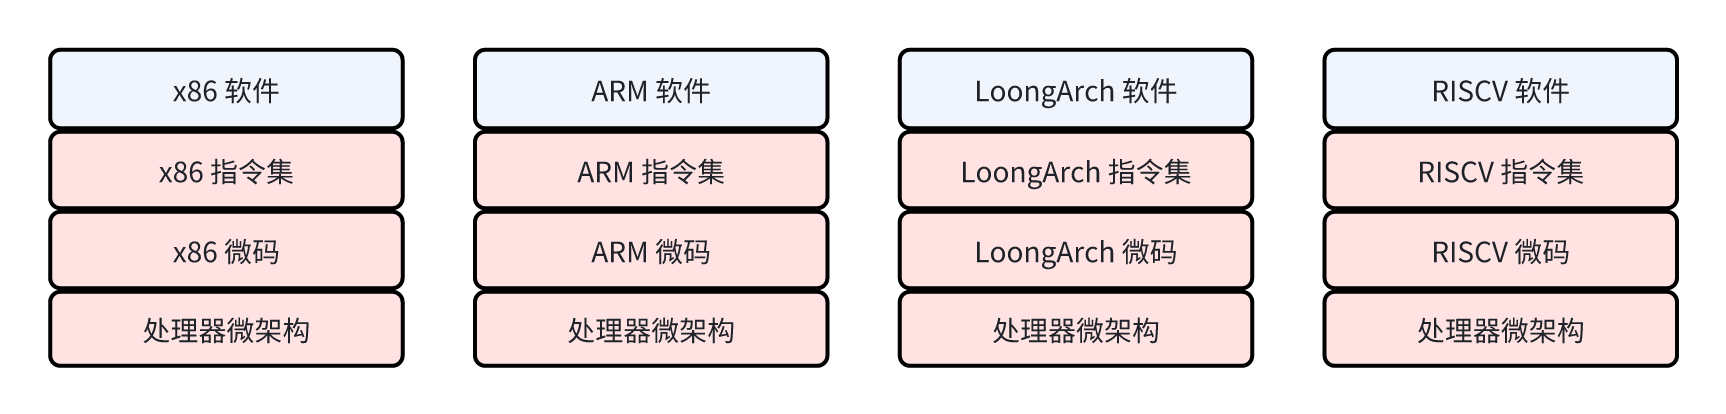
\includegraphics[width=0.8\linewidth]{./image/allCPU_arch.pdf}
    \bicaption{\enspace 不同指令集CPU的架构图}{\enspace Architecture of CPUs with different instruction sets}
    \fignote{图中白色为软件层,红色为硬件层,并忽略了操作系统,这不是本文研究重点。
    对于复杂指令集x86,内部实现了微码层,而精简指令集架构内部一般没有微码层。}
    \label{img:allCPU_arch}
  \end{figure}


如图\ref{img:allCPU_arch}所示,同一套软件源代码需要针对不同的指令集进行编译才能在不同架构的CPU上运行\footnotemark。
而如果软件不能编译,只有二进制程序,就不能在其他架构处理器上运行,这就是生态碎片化问题。
而大量用户态软件处于商业利益、防破解等原因,不会开源,只有二进制程序,这加剧了生态碎片化问题。
例如大量x86版本的工业软件、游戏、办公软件等,只有二进制程序,无法直接在其他架构的CPU上运行。

\footnotetext{这里主要关注C/C++等底层语言,对于Java等支持跨平台运行的语言,也需要Java虚拟机对不同指令集平台进行编译适配。}

随着中国国产处理器的指令集多样化发展,出现了生态碎片化问题,这增加了应用程序在不同架构间迁移和适配的复杂性。存在的问题包括:
    \begin{itemize}
    \item \textbf{适配和迁移负担:} 不同架构间的适配和迁移需要大量人力和物力资源。
    
    \item \textbf{历史兼容包袱:} 不同指令集的历史兼容包袱使得跨架构的兼容性复杂。
    
    \item \textbf{编译与源代码的限制:} 古老软件无源代码,只能通过翻译运行。
    
    \item \textbf{操作系统支持的挑战:} 操作系统厂商需要投入更多资源以支持不同架构。
    \end{itemize}

\section{二进制翻译器概述}
目前,二进制翻译技术是解决生态碎片化问题、兼容性问题的主要方法。

二进制翻译技术能够将源指令集(称为客户指令集, guest ISA)上的二进制程序翻译到目标指令集(称为宿主指令集, host ISA)上执行,
借此能把已有的软件从一个平台迁移到另一个平台,实现不同指令集架构之间的兼容性,丰富新型指令集架构的生态。
在历史上,Alpha\cite{chernoffFX32Profiledirected1998}、Transmeta\cite{dehnertTransmetaCodeMorphing2003}、
Apple\cite{RunningIntelBinaries}、Intel\cite{noauthor_intel_nodate}
等公司都曾经使用过二进制翻译技术来协助推出新的指令集架构,目前市场上也有一些商业化的二进制翻译器产品。

参考一篇二进制翻译综述的分类方法\cite{BT_review},二进制翻译器可以分为静态和动态、用户态和系统态、解释型和翻译型、软件实现和软硬件实现等,
这些分类方式可以根据不同的需求和应用场景进行组合,并且基本是\textbf{正交}的。

下面是对这些分类的简要说明:

\subsection{静态与动态}
静态二进制翻译:在程序执行前,将整个源程序从一种机器指令集转换到另一种。
这种转换通常产生可直接运行的预翻译文件(Ahead-of-Time file, AOT文件),无需在运行时进行额外的转换。
静态翻译的优点在于它可以在转换过程中进行深入的代码分析和优化,但它不适用于即时生成代码(Just-In-Time Code, JIT代码),
也难以处理代码数据混淆等复杂的情况,导致其使用场景受限。

动态二进制翻译:在程序运行时,以基本块或者函数体为单位,
按需将代码从源指令集转换为目标指令集,一边翻译一边执行,这种方法能处理更广泛的情况。
动态翻译还引入了代码缓存(Code Cache),用于存放已经翻译过的代码,以提高性能。
动态翻译过程中能获取更多程序运行时的信息,可以进行更多的优化。
但同时动态翻译也面临着翻译开销大、代码优化不充分等问题。

\begin{figure}[!htbp]
  \centering
  \includegraphics[width=1\linewidth]{./image/sbt_dbt.pdf}
  \bicaption{\enspace 静态与动态二进制翻译器}{\enspace Static and Dynamic Binary Translators}
  \fignote{左图为静态二进制翻译器,在运行前提前翻译成预翻译文件,运行时直接执行。
  右图为动态二进制翻译器,在运行时翻译基本块并存入代码缓存,翻译过的基本块就直接执行。}
  \label{img:sbt_dbt}
\end{figure}

两者的概念图可以查看\ref{img:sbt_dbt}。
目前也有动静结合的方法,即通过静态翻译尽可能翻译更多的基本块并存储在预翻译文件中,
在运行时如果遇到未翻译的基本块再进行动态翻译,这种方法可以减少运行时的翻译开销,提高性能。

\subsection{用户态与系统态}
用户态二进制翻译:仅转换用户空间程序的指令,不涉及操作系统核心态的代码,运行环境可以直接依赖于宿主操作系统。这种翻译对于实现应用程序的跨架构兼容性特别有用,相对于系统态翻译,性能更高。

系统态二进制翻译:模拟整个系统,包括CPU、内存、设备等,能够转换操作系统内核代码和驱动程序,以实现整个操作系统的兼容。这要求翻译器能够处理更为复杂的系统级别的操作,如中断处理和系统调用,通常性能较低。

\begin{figure}[!htbp]
  \centering
  \includegraphics[width=0.8\linewidth]{./image/user_sys.pdf}
  \bicaption{\enspace 用户态与系统态二进制翻译器}{\enspace User and System Binary Translators}
  \label{img:user_sys}
\end{figure}

两者的概念图可以查看\ref{img:user_sys}。

\subsection{解释型与翻译型}
解释型二进制翻译:以单条指令为单位,逐条解释源指令并实时执行。这种方式可以实现较高的兼容性,因为它可以逐步处理源程序的每个指令,但由于不保存已解释的指令,其性能通常较低,比本地原生执行慢10到100倍。一般用于调试、模拟和验证等场景。

翻译型二进制翻译:以基本块为单位,将源程序的指令翻译成目标机器的指令,存储翻译后的基本块,并进行优化,最后执行翻译后的代码。这种方法在翻译阶段可能会花费更多时间,但运行翻译后的代码的速度更快。

\begin{figure}[h]
  \centering
  \includegraphics[width=1\linewidth]{./image/inter_bt.pdf}
  \bicaption{\enspace 解释型与翻译型二进制翻译器}{\enspace Interpretive and Translational Binary Translators}
  \fignote{左图为解释型二进制翻译器,以单条指令为单位,解释指令语义执行。右图为翻译型二进制翻译器,以基本块为单位,翻译整个基本块并进行优化后执行。}
  \label{img:inter_bt}
\end{figure}

两者的概念图可以看\ref{img:inter_bt}。

\subsection{软件实现与软硬件实现}
软件实现:在不修改宿主硬件的情况下,完全在软件层面上实现二进制翻译。这种实现方式的优点在于其灵活性和可移植性,但可能会因为缺乏硬件支持而影响翻译性能。

软硬件实现:结合使用专门的硬件支持和配套的软件技术来提高二进制翻译的效率。例如,通过在处理器中实现特定的硬件间接跳转表(CAM表)来加速间接跳转的翻译执行\cite{Godson3},添加特定的指令集扩展来缩小语义差异\cite{LoongISA}。这种方法可以显著提高性能,但增加了硬件设计的复杂性和成本。

\section{二进制翻译器性能问题}

表\ref{tab:BTs}对这些分类进行了总结,
各种二进制翻译技术的选择取决于特定应用的需求、目标架构的特性以及性能和兼容性之间的权衡。

\begin{table}[!htbp]
  \bicaption{\enspace 二进制翻译技术的分类及优劣势比较}{\enspace Classification and Pros and Cons of Binary Translation Technologies}
  \label{tab:BTs}
\centering
\footnotesize% fontsize
\setlength{\tabcolsep}{4pt}% column separation
\renewcommand{\arraystretch}{1.2}%row space 
  \begin{tabular}{llll}
  \hline
  分类  & 说明                  & 优势           & 不足                  \\ \hline
  静态  & 提前翻译                & 深入的代码分析和优化   & 使用场景受限  \\
  动态  & 运行时翻译和优化            & 能处理动态生成代码    & 额外的运行时开销    \\
  \hline
  用户态 & 只翻译用户态指令            & 实现简单,性能较高    & 支持应用有限     \\
  系统态 &  模拟整个系统 & 能直接跨架构运行操作系统 & 性能较低                \\
  \hline
  解释型 & 逐条指令解释执行            & 方便调试模拟等      & 性能很低 \\
  翻译型 & 以基本块为单位翻译执行       & 性能较高         & 设计更加复杂              \\
  \hline
  软件  & 纯软件实现               & 灵活性和可移植性     & 性能不高                \\
  软硬件 & 特定硬件支持    & 特定硬件加速提升性能   & 增加硬件设计复杂性      \\ \hline   
  \end{tabular}
  \end{table}

目前主流的二进制翻译器主要采用\textbf{动态、用户态、翻译型和软件实现}的方式,如QEMU\cite{bellardQEMUFastPortable2005}、Rosetta2\cite{RosettaTranslationEnvironment, RunningIntelBinaries}、ExaGear\cite{KunPengExaGear}、LATX\cite{LoongArchEnv2022, LoongArch2023}等(Rosetta2也有动静态结合优化,LATX有硬件指令集扩展支持),这是由于动态翻译可以在运行时进行优化并能支持JIT程序的翻译运行,用户态翻译、翻译型翻译可以实现更高的性能,软件实现可以实现更好的可移植性,对硬件修改较少。


% \section{二进制翻译器性能问题}

翻译性能是衡量二进制翻译器优劣的重要指标,
本文将翻译性能定义如下:
\begin{equation}\label{eq:bt_performance}
    \text{翻译性能} = \frac{\text{本地原生代码执行时间}}{\text{基于二进制翻译执行时间}} * 100\%
\end{equation}
对同一份测试程序的源代码用相同编译参数,直接编译到宿主指令集得到原生二进制代码$B_{host}$,
交叉编译到客户指令集得到客户二进制代码$B_{guest}$,
在硬件平台直接运行原生程序$B_{host}$的时间记为\textbf{本地原生代码执行时间}。
使用二进制翻译系统运行客户程序$B_{guest}$的时间记为\textbf{基于二进制翻译执行时间}。
通常后者会大于前者,两者的比值即为翻译性能,性能越高,越接近100\%,说明翻译器越优秀。


但是由于目前主流的二进制翻译器性能相对较低,
例如QEMU\cite{bellardQEMUFastPortable2005}虽然支持多架构应用,但在翻译运行SPEC CPU 2017\cite{SPECCPU2017}程序时候,仅有约10\%的性能。商业二进制翻译器也存在性能损失,
如苹果的Rosetta2\cite{RosettaTranslationEnvironment, RunningIntelBinaries}、
华为的ExaGear\cite{KunPengExaGear}、
和龙芯的LATX\cite{LoongArchEnv2022, LoongArch2023},
性能仅达到原生运行的70\%左右,这直接影响了软件生态迁移的流畅度和成功性,
相对于同架构不同操作系统模拟的虚拟机(性能接近100\%),性能不足也限制了二进制翻译器的广泛应用。
后文\ref{sec:bt_overhead_all}节会详细分析现有二进制翻译器的开销来源。

除了性能问题,二进制翻译也较难实现多架构支持。在虚拟化技术广泛应用的今天,二进制翻译器的多架构支持也是一个重要的研究方向。目前,云计算和移动计算催生出多样化异构系统,计算平台从传统的单一指令系统向多指令系统融合发展,
例如Google使用多种指令集组成的异构系统,
传统的虚拟化只能实现单指令集中多种操作系统的迁移,应用软件难以在不同指令集架构的硬件上迁移运行,
多架构二进制翻译器可以解决跨指令集应用迁移问题。
目前主流的开源二进制翻译器QEMU支持多架构,但性能太低,难以商用化。
探索出高性能的多架构二进制翻译器也是当前的研究热点。

除了CPU架构指令集差异导致的生态碎片化,GPU目前也面临相似的问题。
英伟达公司的CUDA软件生态在GPU领域占据绝对优势,但是只支持英伟达的GPU。
AMD、Intel和很多国内显卡公司开发的加速器无法直接运行CUDA程序,这也导致了GPU生态碎片化问题。
随着更多有竞争力的GPU架构的出现,也有更多用户倾向于在不同GPU架构上运行CUDA程序,目前有两种解决方案:
重新编译CUDA程序,或者通过二进制兼容技术。
重新编译现有的 CUDA 程序完全合法但需要人力投入,例如AMD 和 Intel 都有工具分别将 CUDA 程序移植到他们的 ROCm和 OneAPI平台。
而后者的代表是ZLUDA\cite{ZLUDA},通过兼容层允许在非英伟达GPU上运行未经修改的CUDA程序
(兼容层和二进制翻译不同,更接近于Wine这样的库兼容技术),
并声称提供了“接近原生”的性能。但最新版本的英伟达用户协议(ELUA)中明确禁止使用ZLUDA等技术在其他平台上运行CUDA代码,
但这并不代表兼容技术不可行,也有更多技术被提出用以打破“CUDA霸权”。
但本文的关注点在于CPU架构的二进制翻译技术,对于GPU架构的二进制兼容技术暂不做更多讨论。



% \section{多架构软硬协同二进制翻译的需求}
\section{本文的主要工作及贡献}

为了解决CPU\textbf{生态碎片化}问题和\textbf{二进制翻译器性能}问题,需要一种多架构软硬协同的二进制翻译技术。这项技术的关键目标是在同一套硬件下实现多指令集的共存,同时实现接近原生的运行效率。

如图\ref{img:my_arch}所示,本课题组提出了一种多架构软硬协同的二进制翻译技术——\textbf{微译器},按照上述分类属于动静结合、用户态、翻译型、软硬结合,
通过在硬件层面支持一套融合微码,在软件层面实现多架构的二进制翻译器,进而能实现多种指令集软件的共存和运行,
同时性能接近原生运行性能。


\begin{figure}[!htbp]
    \centering
    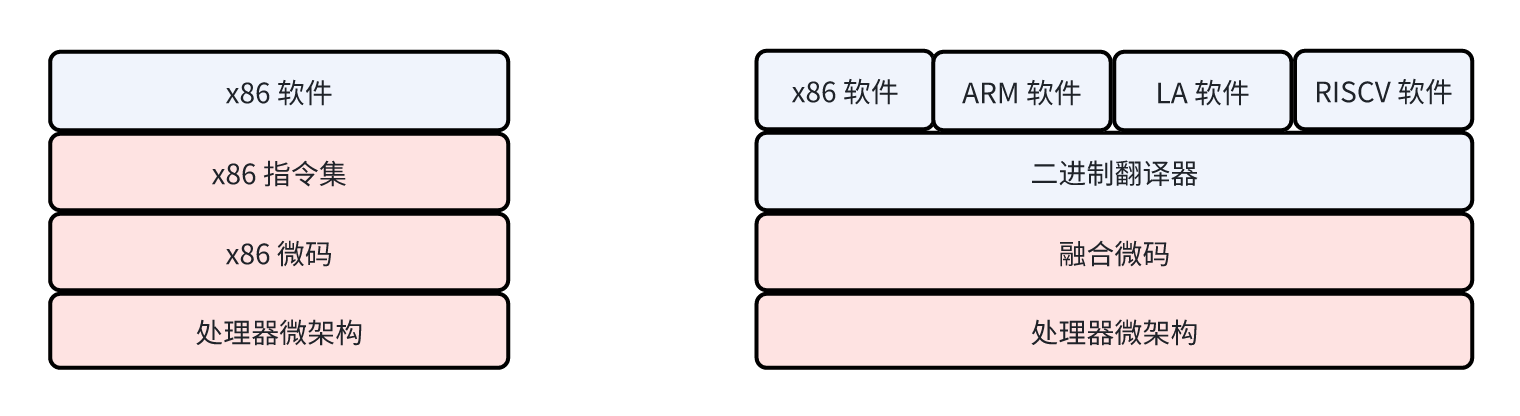
\includegraphics[width=0.6\linewidth]{./image/my_arch.pdf}
    \bicaption{\enspace 微译器架构简图}{\enspace The architecture of Micro-Translator}
    \fignote{硬件仅对外暴露微码,软件二进制翻译器支持多架构,性能接近原生运行性能。}
    \label{img:my_arch}
  \end{figure}

% 这项技术的优势在于:

% 1. \textbf{打破指令集边界,消除应用迁移成本:} 应用程序无需适配和迁移至特定指令集,可直接在同一套硬件上运行,降低了软件开发和维护的复杂性。

% 2. \textbf{硬件对外暴露微码,规避x86等授权问题:} 通过在硬件层面暴露微码,技术在一定程度上规避了x86等架构的授权问题,提高了国产处理器的自主性。

% 3. \textbf{软件维护历史兼容,微码迭代优化:} 软件层的二进制翻译器维护历史兼容性,硬件层微码可以迭代优化,
% 进而适配更多指令集或者提高性能,二进制翻译器都可以屏蔽这些变化,保持软件的兼容性。

在本团队的工作基础上,
\textbf{本文}在微译器已有的支持x86指令集翻译执行的框架下,添加了RISC-V架构的支持,
本文的主要工作及贡献如下:

1. 设计并实现了RISC-V微译器:设计了寄存器映射方案,累计添加了51条微码指令用于支持272条RISC-V指令集的翻译执行。
实现了微译器对于多架构的高效支持,为添加更多指令集提供了技术支持。

2. 优化了RISC-V微译器的性能:添加了4种优化方案,包括行尾放松、分支放松、可变长行、指令压缩。
这些优化方案进一步提升了翻译缓存的利用率,降低了缓存缺失率,提升了微译器整体性能。

本文在Gem5模拟器中实现了RISC-V微译器原型系统,
实验显示优化后的RISC-V微译器在运行SPEC 2000测试的平均性能达到了原生程序的96.1\%,
有效缓解了性能瓶颈,实现了接近原生程序的运行效率。微译器同时支持x86和RISC-V两种指令集,
能有效的解决CPU生态碎片化问题和二进制翻译器性能问题,
为多架构二进制翻译提供了一种新的解决方案。

\section{论文的组织结构}
% 本文在第二章介绍二进制翻译相关工作,包括软硬协同二进制翻译器和纯软件二进制翻译器。第三章介绍微译器的架构设计和实现,第四章介绍在微译器中添加RISC-V架构的实现,第五章介绍微译器优化方案,第六章介绍微译器的性能测试和分析,第七章总结全文并展望未来工作。

本文的组织结构如下:

在第二章介绍二进制翻译的相关工作,包括4种主流的软件二进制翻译器,发现其性能难以接近原生性能。
接下来对软件二进制翻译器的性能开销进行分析,
然后介绍一些已有的软硬协同二进制翻译器是如何缓解性能瓶颈的,
为了更进一步降低性能开销,引出了复杂指令集x86处理器中微码缓存的概念,
最后介绍团队项目——微译器的架构设计和实现,并讲解微译器是如何消除间接跳转的性能开销,进而提升翻译性能。

第三章介绍本文在微译器中添加RISC-V架构的设计与实现,
首先讲解了软件层二进制翻译器如何重构用于支持多架构翻译,
接下来详细介绍融合微码编码设计来更好的提取不同指令集的共性和差异,
进而分析RISC-V和x86的指令集语义差异,如何添加合适的融合微码指令用以支持RISC-V指令翻译。
最后分析RISC-V和x86 ABI差异,如何在RISC-V微译器中处理系统调用差异、寄存器映射、栈的初始化问题等。

第四章介绍RISC-V微译器的优化方案,
RISC-V微译器在引入翻译缓存后会产生额外的硬件性能开销。
本章首先分析这部分性能开销的来源,然后提出了几种优化方案,
包括行尾放松、分支放松、可变长行、指令压缩,这些优化方案降低了RISC-V微译器的性能开销,提升了整体性能。

第五章介绍RISC-V微译器的实验数据分析,包括搭建原型系统使用的Gem5实验环境,运行性能分析使用的测试程序,
进行正确性验证使用的调试环境,然后对RISC-V微译器的性能进行测试和分析,并分别统计了各种优化方案的性能提升。

第六章总结全文并展望未来工作。
